\documentclass[12pt]{dalcsthesis}
\usepackage{graphicx}
\graphicspath{ {images/} }
\begin{document}
\mcs 
\title{Bridging Data and Electronic Dance Music}
\author{Jasdev Singh}
\defenceday{9}
\defencemonth{March}
\defenceyear{2014}
\convocation{May}{2014}

\supervisor{Dr. Yanjun Qi}
\reader{Matthew N. Eisler, PhD}

\nolistoftables
\nolistoffigures

\frontmatter

\begin{abstract}
Electronic dance music (EDM) is a relatively new genre with unique features such as a myriad of subgenres and the common notion of playing live events in a festival format. With its rise to mainstream popularity, there are opportunities to explore the social dynamics of EDM by analyzing datasets associated with the genre. In our research, we seek to understand three such public datasets, the DJ Magazine Top 100, Electric Zoo Festival set lists, and SoundCloud comment data, at a deeper level. Some of the techniques employed are time-series analyses, network diagrams, and sentiment analysis, to help draw conclusions about this young, but rapidly growing, genre.
\end{abstract}

\begin{acknowledgements}
\begin{itemize}
	\item Dr. Yanjun Qi, PhD
	\item Matthew N. Eisler, PhD
	\item UVa's Association of Computing Machinery
\end{itemize}
\end{acknowledgements}

\mainmatter

\chapter{Introduction}

\section{Background}

Electronic dance music (often called EDM) includes multiple electronic music genres, usually for dance-based events (festivals or clubs). At these live events, it is very common for dee jays (DJs) to play continuous sets, ranging from 30 minute to multiple hour mixes. Moreover, producers and DJs will often collaborate on and play each other's music. Below is a graph from a recent report by Google Music's Research Group [citation] showing the popularity of various genres uploaded to the Google Play store [link], since the service's inception. Highlighted by the red box is Dance and Electronic music. It can be seen that EDM is roughly the 6th largest genre, as of the most recent year in the survey.

\begin{figure}[h]
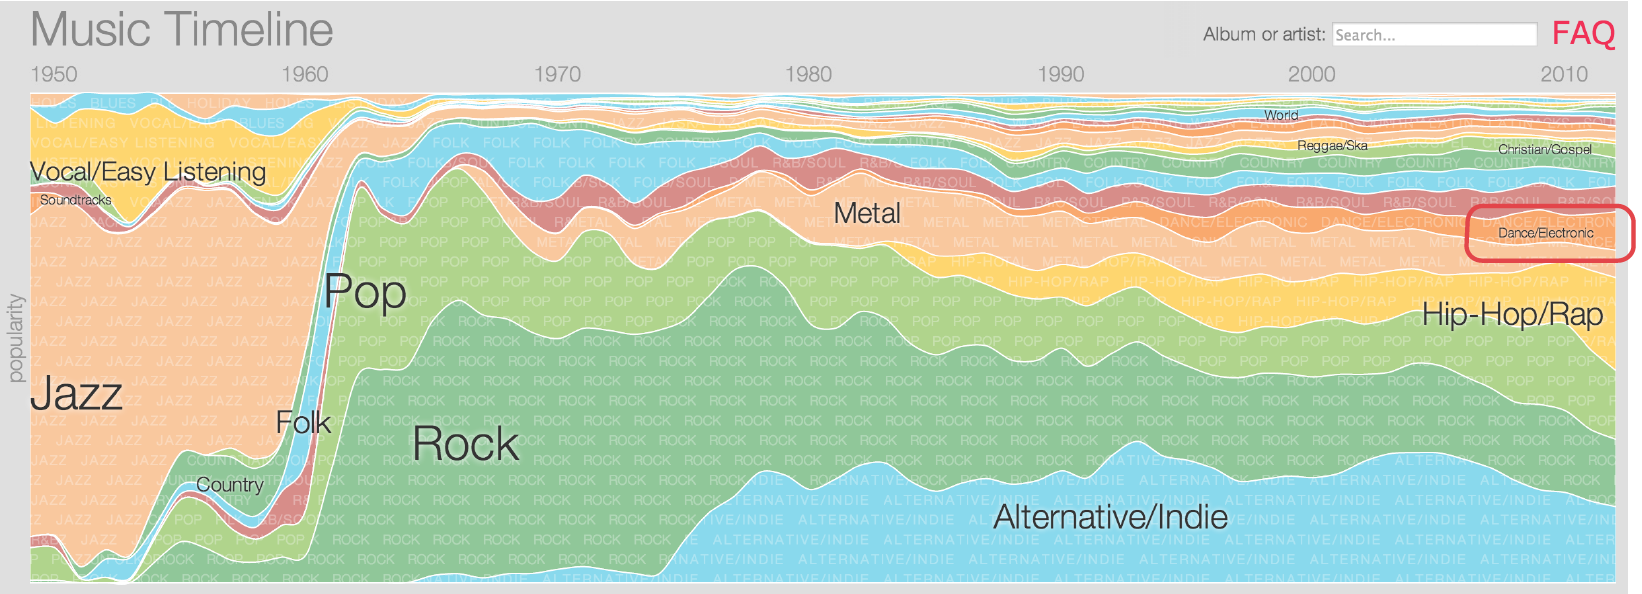
\includegraphics[scale=.49]{genre_graph}
\centering
\end{figure}

A unique feature of dance music is the wide array of subgenres present. This allows for the rise of communities of producers and opportunities for remixing originals into other subgenres. Zooming in on the graph presented previously, we can see just how diversified the overall genre is, with notable examples being trance, techno, house, ambient, and drum \& bass. \newpage

\begin{figure}[h]
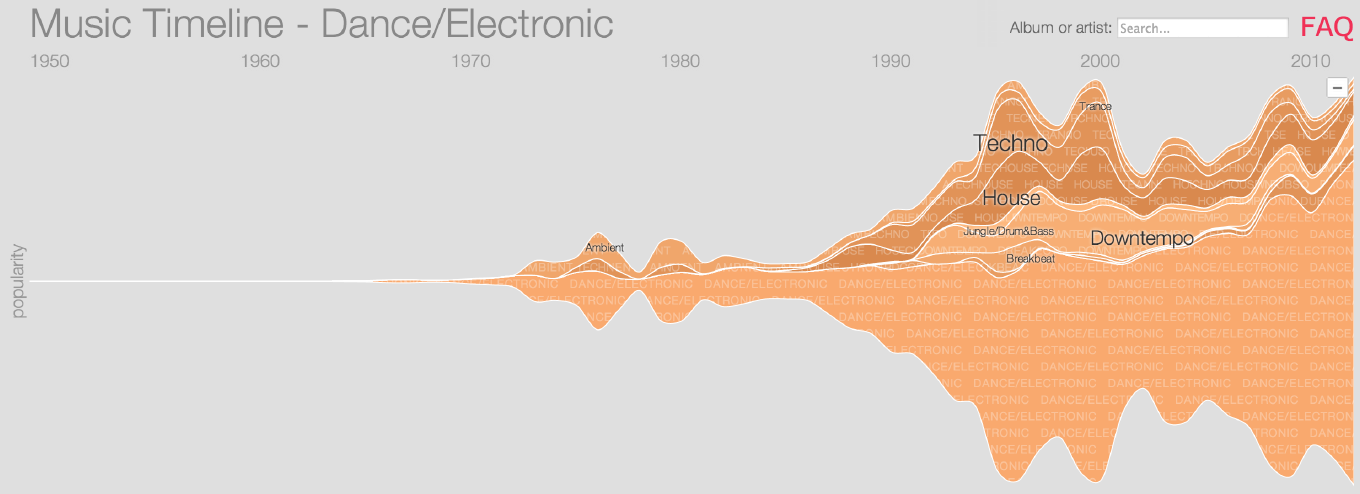
\includegraphics[scale=.65]{subgenre_graph}
\centering
\end{figure}

Next up, we will highlight some of the most popular genres within EDM. To begin, House is a genre typically noted by a 4/4 kick drum and a 120 - 130 beats per minute (bpm) range. Some common names within House are Avicii, Swedish House Mafia, and David Guetta. While bucketing artists into genres is not completely black and white, one can generally place artists in certain buckets based on the majority of their productions. Secondly, Electro is a style with identifiable synths and a tempo range of 125 - 135 bpm. Some notable artists in the space are Dada Life, Justice, and Boy's Noize. Third is Dubstep, defined by an oscillating wobble bass. The bpm range hovers around 140 and big producers in the genre are Skrillex, Bassnectar, Skream, and Benga. Lastly, Trance is another large subgenre. It's tempo range is wide, 125 - 150 bpm, and is noted by anthems and exaggerated builds. Trance has been doing extremely well in the DJ Magazine Top 100, which we will introduce soon, and is lead by artists such as Armin van Buuren, Above \& Beyond, and Ferry Corsten.

\section{Motivation}

Being a relatively young genre, there has not been a lot of research done on the EDM social demographic and artists. In this paper, we will take a look at three datasets from an analytical perspective. To start, we will note trends in the DJ Magazine Top 100 poll, which is an attempt to put a stack rank on DJs and producers from year to year. Secondly, we will look at set lists of what DJs played at live events, specifically one festival in New York called Electric Zoo. From these set lists, we can make connections from specific DJs to others by how they played and/or remixed each other's work. Such connections naturally lead to the formation of a network diagram. Lastly, we will use sentiment analysis to gain insights from public user comments on music hosted on the popular online streaming service, SoundCloud. From the text data housed in these timestamped comments, we will see the effectiveness in making conclusions in the underlying audio.

\chapter{Previous Work}

Previous wok in the realm of analyzing data on EDM is far and in between. However, Eventbrite, an online ticketing platform for many live events, put out a study in June 2013 showcasing behavioral trends on how EDM listeners shared content on social media before and after events. [Add more details on the study and connection]

\chapter{Framework}

\section{DJ Magazine Top 100}

Starting in 1997, DJ Magazine has put together a popular vote poll to determine the top 100 DJs each year. However, when it comes to subjective topics, like music, this type of poll has received criticism since popularity does not always coincide with musical talent. But, on a higher level, we can use this time series data to draw larger and more general conclusions about the genre and its constituents. In our study, we scraped the poll data and made then available in both CSV [link] and JSON [link] format. 

\section{Top 100 Case Study \#1, Swedish House Mafia}

To exemplify some of the trends in these charts, we begin with the DJ trio that is Swedish House Mafia. Starting in 2008, Steve Angello, Sebastian Ingrosso, and Axwell began touring around the world together and recently stopped in 2013. Below is a plot of their respective rankings in the chart, including the ranking of the group overall: \newpage

\begin{figure}[h]
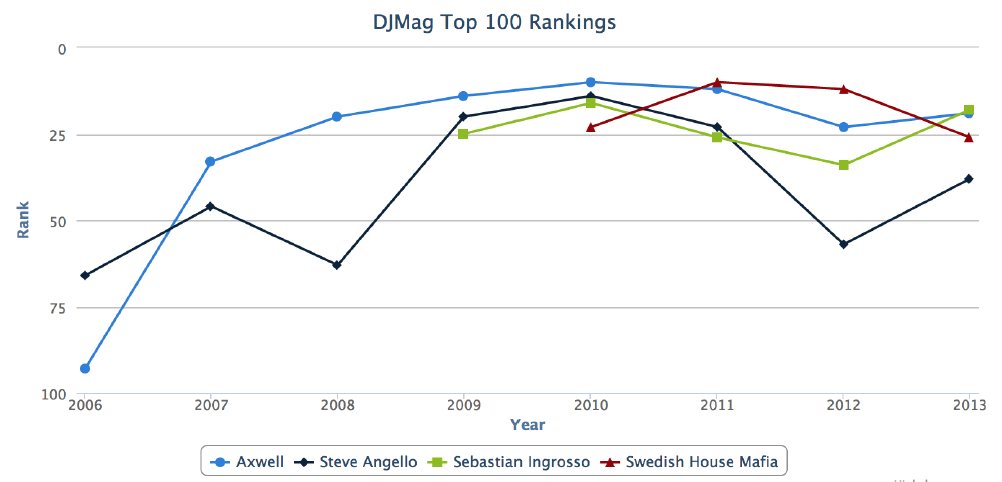
\includegraphics[scale=.65]{shm_graph}
\centering
\end{figure}

From this figure, we can see that upon the group' splitting in 2013, both Sebastian Ingrosso and Axwell had higher rankings in the poll, even above the group, whereas Steve Angello's regard in the public eye was ranked lower. The reasoning for the group's spit is unknown (although a documentary [link] is set to be released soon), but this may help us gain some insight on the situation.

\section{Top 100 Case Study \#2, Trance Rankings}

Trance is an extremely popular electronic genre that has typically held a strong showing in the polls. However, recently in 2013, there has been some pushback from fans against the genre as DJs and producers have been experimenting with more "radio" style tracks. Below we have a plot of all the trance DJs appearing in the Top 100:

\begin{figure}[h]
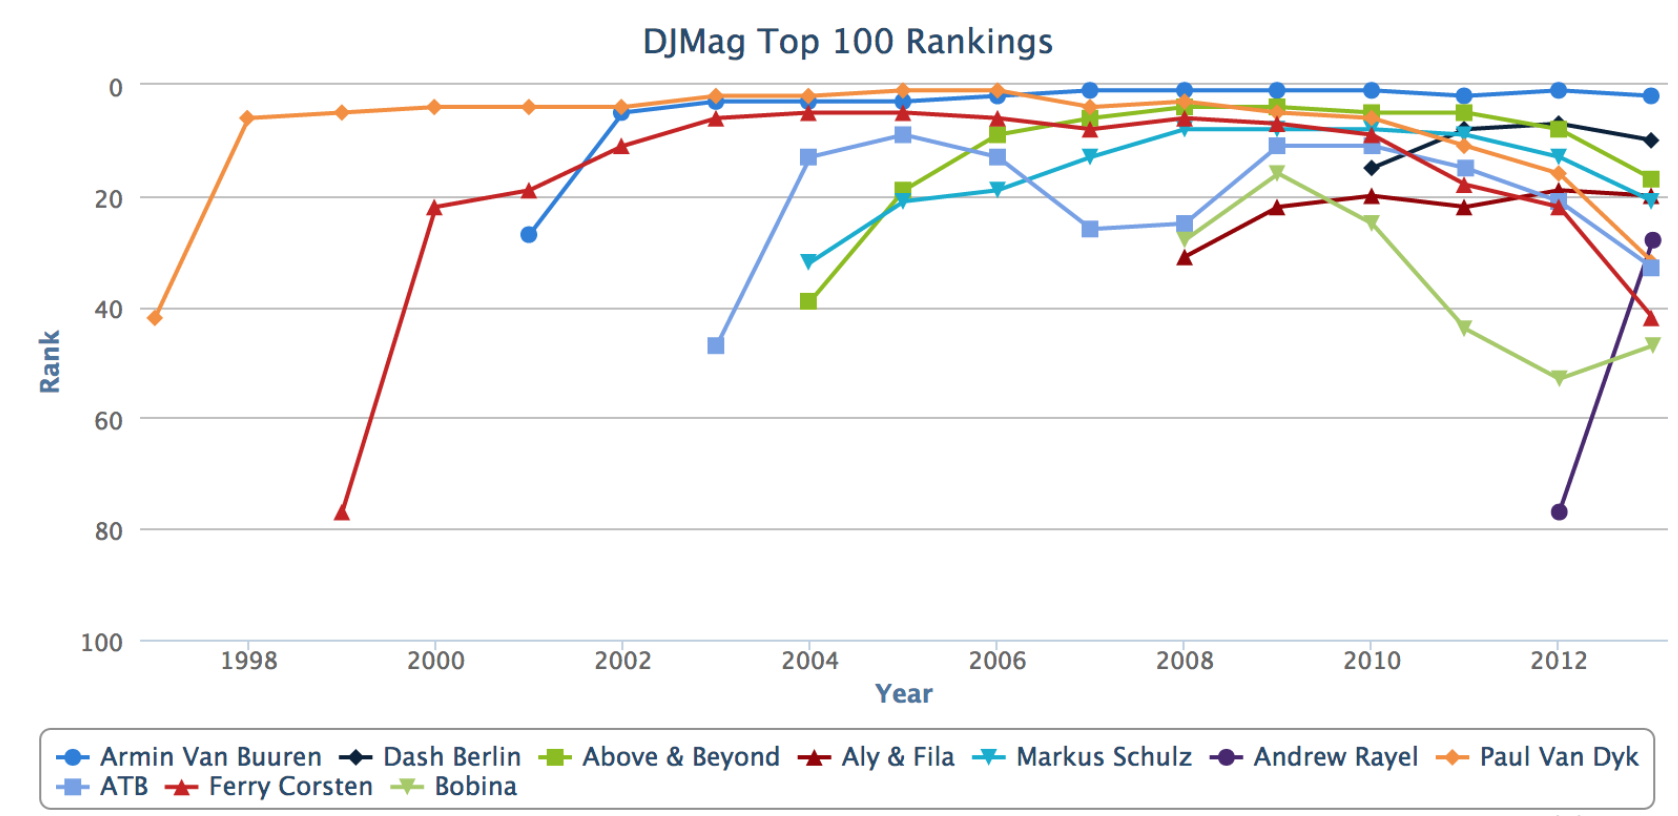
\includegraphics[scale=.4]{trance_graph}
\centering
\end{figure}

In 2013, every DJ in the poll, with the exception of Bobina and Andrew Rayel, actually dipped in ranking, when compared to the previous years.

\section{Top 100 Case Study \#3, Mentor Rankings}



\chapter{Conclusion}
\chapter{Future Work}

\bibliographystyle{plain}
\bibliography{simple}

\end{document}
